As for the experiment, the concept of "cashier-free supermarket" can be achieved by our simulator scene.
And we can make good use of our experimental results in small and medium-sized supermarkets.
By investigating supermarkets on the market, such as 7-11, Family, GIANT.
Most of them can use the multi camera recognition system, and shown in Fig.12

\begin{figure}[htbp]
\centerline{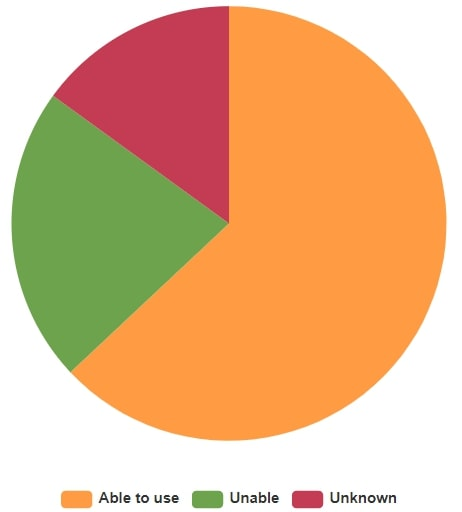
\includegraphics[width=3cm,scale=0.3]{pie.jpg}}
\caption{Through our survey, the supermarkets whether can use our identification system}
\label{fig}
\end{figure}

In the pie chart, 63\% supermarket can use the recognition system directly.
11\% supermarkets may be unavailable due to shelf placement or small area.
According to the survey, most supermarkets can use this recognition system.

However, there are many problems to be solved meanwhile.
When there are too many people in the supermarket, they will interfere with camera shooting.
How to identify two objects with the same weight and very similar weight accurately.
These are the problems we need to solve in the future.
